% Options for packages loaded elsewhere
\PassOptionsToPackage{unicode}{hyperref}
\PassOptionsToPackage{hyphens}{url}
%
\documentclass[
]{article}
\usepackage{amsmath,amssymb}
\usepackage{lmodern}
\usepackage{iftex}
\ifPDFTeX
  \usepackage[T1]{fontenc}
  \usepackage[utf8]{inputenc}
  \usepackage{textcomp} % provide euro and other symbols
\else % if luatex or xetex
  \usepackage{unicode-math}
  \defaultfontfeatures{Scale=MatchLowercase}
  \defaultfontfeatures[\rmfamily]{Ligatures=TeX,Scale=1}
\fi
% Use upquote if available, for straight quotes in verbatim environments
\IfFileExists{upquote.sty}{\usepackage{upquote}}{}
\IfFileExists{microtype.sty}{% use microtype if available
  \usepackage[]{microtype}
  \UseMicrotypeSet[protrusion]{basicmath} % disable protrusion for tt fonts
}{}
\makeatletter
\@ifundefined{KOMAClassName}{% if non-KOMA class
  \IfFileExists{parskip.sty}{%
    \usepackage{parskip}
  }{% else
    \setlength{\parindent}{0pt}
    \setlength{\parskip}{6pt plus 2pt minus 1pt}}
}{% if KOMA class
  \KOMAoptions{parskip=half}}
\makeatother
\usepackage{xcolor}
\IfFileExists{xurl.sty}{\usepackage{xurl}}{} % add URL line breaks if available
\IfFileExists{bookmark.sty}{\usepackage{bookmark}}{\usepackage{hyperref}}
\hypersetup{
  pdftitle={Homework - Week 8},
  pdfauthor={Caio Geraldes},
  hidelinks,
  pdfcreator={LaTeX via pandoc}}
\urlstyle{same} % disable monospaced font for URLs
\usepackage[margin=1in]{geometry}
\usepackage{color}
\usepackage{fancyvrb}
\newcommand{\VerbBar}{|}
\newcommand{\VERB}{\Verb[commandchars=\\\{\}]}
\DefineVerbatimEnvironment{Highlighting}{Verbatim}{commandchars=\\\{\}}
% Add ',fontsize=\small' for more characters per line
\usepackage{framed}
\definecolor{shadecolor}{RGB}{248,248,248}
\newenvironment{Shaded}{\begin{snugshade}}{\end{snugshade}}
\newcommand{\AlertTok}[1]{\textcolor[rgb]{0.94,0.16,0.16}{#1}}
\newcommand{\AnnotationTok}[1]{\textcolor[rgb]{0.56,0.35,0.01}{\textbf{\textit{#1}}}}
\newcommand{\AttributeTok}[1]{\textcolor[rgb]{0.77,0.63,0.00}{#1}}
\newcommand{\BaseNTok}[1]{\textcolor[rgb]{0.00,0.00,0.81}{#1}}
\newcommand{\BuiltInTok}[1]{#1}
\newcommand{\CharTok}[1]{\textcolor[rgb]{0.31,0.60,0.02}{#1}}
\newcommand{\CommentTok}[1]{\textcolor[rgb]{0.56,0.35,0.01}{\textit{#1}}}
\newcommand{\CommentVarTok}[1]{\textcolor[rgb]{0.56,0.35,0.01}{\textbf{\textit{#1}}}}
\newcommand{\ConstantTok}[1]{\textcolor[rgb]{0.00,0.00,0.00}{#1}}
\newcommand{\ControlFlowTok}[1]{\textcolor[rgb]{0.13,0.29,0.53}{\textbf{#1}}}
\newcommand{\DataTypeTok}[1]{\textcolor[rgb]{0.13,0.29,0.53}{#1}}
\newcommand{\DecValTok}[1]{\textcolor[rgb]{0.00,0.00,0.81}{#1}}
\newcommand{\DocumentationTok}[1]{\textcolor[rgb]{0.56,0.35,0.01}{\textbf{\textit{#1}}}}
\newcommand{\ErrorTok}[1]{\textcolor[rgb]{0.64,0.00,0.00}{\textbf{#1}}}
\newcommand{\ExtensionTok}[1]{#1}
\newcommand{\FloatTok}[1]{\textcolor[rgb]{0.00,0.00,0.81}{#1}}
\newcommand{\FunctionTok}[1]{\textcolor[rgb]{0.00,0.00,0.00}{#1}}
\newcommand{\ImportTok}[1]{#1}
\newcommand{\InformationTok}[1]{\textcolor[rgb]{0.56,0.35,0.01}{\textbf{\textit{#1}}}}
\newcommand{\KeywordTok}[1]{\textcolor[rgb]{0.13,0.29,0.53}{\textbf{#1}}}
\newcommand{\NormalTok}[1]{#1}
\newcommand{\OperatorTok}[1]{\textcolor[rgb]{0.81,0.36,0.00}{\textbf{#1}}}
\newcommand{\OtherTok}[1]{\textcolor[rgb]{0.56,0.35,0.01}{#1}}
\newcommand{\PreprocessorTok}[1]{\textcolor[rgb]{0.56,0.35,0.01}{\textit{#1}}}
\newcommand{\RegionMarkerTok}[1]{#1}
\newcommand{\SpecialCharTok}[1]{\textcolor[rgb]{0.00,0.00,0.00}{#1}}
\newcommand{\SpecialStringTok}[1]{\textcolor[rgb]{0.31,0.60,0.02}{#1}}
\newcommand{\StringTok}[1]{\textcolor[rgb]{0.31,0.60,0.02}{#1}}
\newcommand{\VariableTok}[1]{\textcolor[rgb]{0.00,0.00,0.00}{#1}}
\newcommand{\VerbatimStringTok}[1]{\textcolor[rgb]{0.31,0.60,0.02}{#1}}
\newcommand{\WarningTok}[1]{\textcolor[rgb]{0.56,0.35,0.01}{\textbf{\textit{#1}}}}
\usepackage{graphicx}
\makeatletter
\def\maxwidth{\ifdim\Gin@nat@width>\linewidth\linewidth\else\Gin@nat@width\fi}
\def\maxheight{\ifdim\Gin@nat@height>\textheight\textheight\else\Gin@nat@height\fi}
\makeatother
% Scale images if necessary, so that they will not overflow the page
% margins by default, and it is still possible to overwrite the defaults
% using explicit options in \includegraphics[width, height, ...]{}
\setkeys{Gin}{width=\maxwidth,height=\maxheight,keepaspectratio}
% Set default figure placement to htbp
\makeatletter
\def\fps@figure{htbp}
\makeatother
\setlength{\emergencystretch}{3em} % prevent overfull lines
\providecommand{\tightlist}{%
  \setlength{\itemsep}{0pt}\setlength{\parskip}{0pt}}
\setcounter{secnumdepth}{-\maxdimen} % remove section numbering
\ifLuaTeX
  \usepackage{selnolig}  % disable illegal ligatures
\fi

\title{Homework - Week 8}
\author{Caio Geraldes}
\date{}

\begin{document}
\maketitle

The data in \texttt{week08\_Monks.csv} (found on the course website) are
``like'' and ``dislike'' nominations by 18 monks living in the same
monastery over three time periods. Therefore the observed variables are
counts from 0 to 3 of times monk A nominated monk B as liked or
disliked.1 Each row in the data is a pair of monks (a dyad). The
variables are:

\begin{itemize}
\tightlist
\item
  A: Index number for first monk in dyad
\item
  B: Index number for second monk in dyad
\item
  like\_AB: Number of times A nominated B as liked
\item
  like\_BA: Number of times B nominated A as liked
\item
  dislike\_AB: Number of times A nominated B as disliked
\item
  dislike\_BA: Number of times B nominated A as disliked
\end{itemize}

\begin{Shaded}
\begin{Highlighting}[]
\NormalTok{monks }\OtherTok{\textless{}{-}} \FunctionTok{read\_csv}\NormalTok{(}\StringTok{"./week08\_Monks.csv"}\NormalTok{, }\AttributeTok{show\_col\_types =} \ConstantTok{FALSE}\NormalTok{)}

\NormalTok{dat }\OtherTok{\textless{}{-}} \FunctionTok{list}\NormalTok{(}
    \AttributeTok{N =} \FunctionTok{nrow}\NormalTok{(monks),}
    \AttributeTok{D =}\NormalTok{ monks}\SpecialCharTok{$}\NormalTok{dyad\_id,}
    \AttributeTok{mA =}\NormalTok{ monks}\SpecialCharTok{$}\NormalTok{A,}
    \AttributeTok{mB =}\NormalTok{ monks}\SpecialCharTok{$}\NormalTok{B,}
    \AttributeTok{LAB =}\NormalTok{ monks}\SpecialCharTok{$}\NormalTok{like\_AB,}
    \AttributeTok{LBA =}\NormalTok{ monks}\SpecialCharTok{$}\NormalTok{like\_BA,}
    \AttributeTok{DAB =}\NormalTok{ monks}\SpecialCharTok{$}\NormalTok{dislike\_AB,}
    \AttributeTok{DBA =}\NormalTok{ monks}\SpecialCharTok{$}\NormalTok{dislike\_BA}
\NormalTok{)}
\end{Highlighting}
\end{Shaded}

\hypertarget{question-1}{%
\section{Question 1}\label{question-1}}

Use these data to estimate the amount of reciprocity in ``like''
nominations within dyads. You can ignore the ``dislike'' data for now.
Use the social network example from the book to help, but you should
modify it appropriately.

\hypertarget{answer}{%
\subsection{Answer}\label{answer}}

We define a model where the number of like votes from A to B, \(L_{AB}\)
is a binomial distribution of size 3 and probability \(p_{L_{AB}}\),
with symmetric values indexed for the direction \(B \rightarrow A\). The
logit of a \(p_{L_j}\) is the sum of an intercept \(\alpha\) with an
effect of the positive ties \(T^+\) for \(A \rightarrow B\), correlated
to its counterpart for \(B \rightarrow A\). The priors are fairly flat.

\[
\begin{aligned}
    L_{AB} \sim \text{Binomial}(3, p_{L_{AB}})\\
    L_{BA} \sim \text{Binomial}(3, p_{L_{BA}})\\
    \text{logit}(p_{L_{AB}}) = \alpha + T^+_{AB_i}\\
    \text{logit}(p_{L_{BA}}) = \alpha + T^+_{BA_i}\\
    \alpha \sim \text{Normal}(0,1)\\
    \begin{pmatrix}T^+_{AB}\\T^+_{BA}\end{pmatrix} \sim \text{MVNormal}\begin{pmatrix}\begin{pmatrix}0\\0\end{pmatrix}, \begin{pmatrix}\sigma_{T^+}^2 & \rho_{T^+}\sigma_{T^+}^2\\\rho_{T^+}\sigma_{T^+}^2 &\sigma_{T^+}^2\end{pmatrix}\end{pmatrix}\\
    \sigma_{T^+} \sim \text{Exponential}(1)\\
    \rho_{T^+} \sim \text{LKJCorr}(2)
\end{aligned}
\]

\begin{Shaded}
\begin{Highlighting}[]
\NormalTok{f.m1 }\OtherTok{\textless{}{-}} \FunctionTok{alist}\NormalTok{(}
\NormalTok{    LAB }\SpecialCharTok{\textasciitilde{}} \FunctionTok{binomial}\NormalTok{(}\DecValTok{3}\NormalTok{, pLAB),}
\NormalTok{    LBA }\SpecialCharTok{\textasciitilde{}} \FunctionTok{binomial}\NormalTok{(}\DecValTok{3}\NormalTok{, pLBA),}

    \FunctionTok{logit}\NormalTok{(pLAB) }\OtherTok{\textless{}{-}}\NormalTok{ a }\SpecialCharTok{+}\NormalTok{ pT[D,}\DecValTok{1}\NormalTok{],}
    \FunctionTok{logit}\NormalTok{(pLBA) }\OtherTok{\textless{}{-}}\NormalTok{ a }\SpecialCharTok{+}\NormalTok{ pT[D,}\DecValTok{2}\NormalTok{],}

\NormalTok{    a }\SpecialCharTok{\textasciitilde{}} \FunctionTok{normal}\NormalTok{(}\DecValTok{0}\NormalTok{,}\DecValTok{1}\NormalTok{),}

\NormalTok{    transpars}\SpecialCharTok{\textgreater{}}\NormalTok{ matrix[N,}\DecValTok{2}\NormalTok{]}\SpecialCharTok{:}\NormalTok{pT }\OtherTok{\textless{}{-}} 
        \FunctionTok{compose\_noncentered}\NormalTok{(}\FunctionTok{rep\_vector}\NormalTok{(sigma\_pT, }\DecValTok{2}\NormalTok{), L\_Rho\_pT, z),}
\NormalTok{    matrix[}\DecValTok{2}\NormalTok{,N]}\SpecialCharTok{:}\NormalTok{z }\SpecialCharTok{\textasciitilde{}} \FunctionTok{normal}\NormalTok{(}\DecValTok{0}\NormalTok{,}\DecValTok{1}\NormalTok{),}
\NormalTok{    cholesky\_factor\_corr[}\DecValTok{2}\NormalTok{]}\SpecialCharTok{:}\NormalTok{L\_Rho\_pT }\SpecialCharTok{\textasciitilde{}} \FunctionTok{lkj\_corr\_cholesky}\NormalTok{(}\DecValTok{2}\NormalTok{),}
\NormalTok{    sigma\_pT }\SpecialCharTok{\textasciitilde{}} \FunctionTok{exponential}\NormalTok{(}\DecValTok{1}\NormalTok{),}

\NormalTok{    gq}\SpecialCharTok{\textgreater{}}\NormalTok{ matrix[}\DecValTok{2}\NormalTok{,}\DecValTok{2}\NormalTok{]}\SpecialCharTok{:}\NormalTok{Rho\_pT }\OtherTok{\textless{}\textless{}{-}} \FunctionTok{Chol\_to\_Corr}\NormalTok{(L\_Rho\_pT)}
\NormalTok{)}

\NormalTok{m1 }\OtherTok{\textless{}{-}} \FunctionTok{ulam}\NormalTok{(}
    \AttributeTok{flist =}\NormalTok{ f.m1,}
    \AttributeTok{data =}\NormalTok{ dat,}
    \AttributeTok{chains=}\DecValTok{4}\NormalTok{,}
    \AttributeTok{cores=}\DecValTok{4}\NormalTok{,}
    \AttributeTok{iter=}\DecValTok{2000}\NormalTok{,}
    \AttributeTok{log\_lik=}\ConstantTok{TRUE}\NormalTok{,}
    \AttributeTok{file=}\StringTok{"./models/m1"}\NormalTok{)}
\end{Highlighting}
\end{Shaded}

\begin{Shaded}
\begin{Highlighting}[]
\FunctionTok{precis}\NormalTok{(m1, }\AttributeTok{pars=}\FunctionTok{c}\NormalTok{(}\StringTok{"a"}\NormalTok{, }\StringTok{"sigma\_pT"}\NormalTok{, }\StringTok{"Rho\_pT"}\NormalTok{), }\AttributeTok{depth=}\DecValTok{3}\NormalTok{)}
\end{Highlighting}
\end{Shaded}

\begin{verbatim}
##                   mean        sd       5.5%      94.5%    n_eff    Rhat4
## a           -4.1998182 0.4222707 -4.9002953 -3.5552142 2724.439 1.000317
## sigma_pT     3.4172822 0.4293001  2.7851249  4.1354549 1748.562 1.001322
## Rho_pT[1,1]  1.0000000 0.0000000  1.0000000  1.0000000      NaN      NaN
## Rho_pT[1,2]  0.6304678 0.1047167  0.4491242  0.7826848 1206.704 1.001078
## Rho_pT[2,1]  0.6304678 0.1047167  0.4491242  0.7826848 1206.704 1.001078
## Rho_pT[2,2]  1.0000000 0.0000000  1.0000000  1.0000000      NaN      NaN
\end{verbatim}

\begin{center}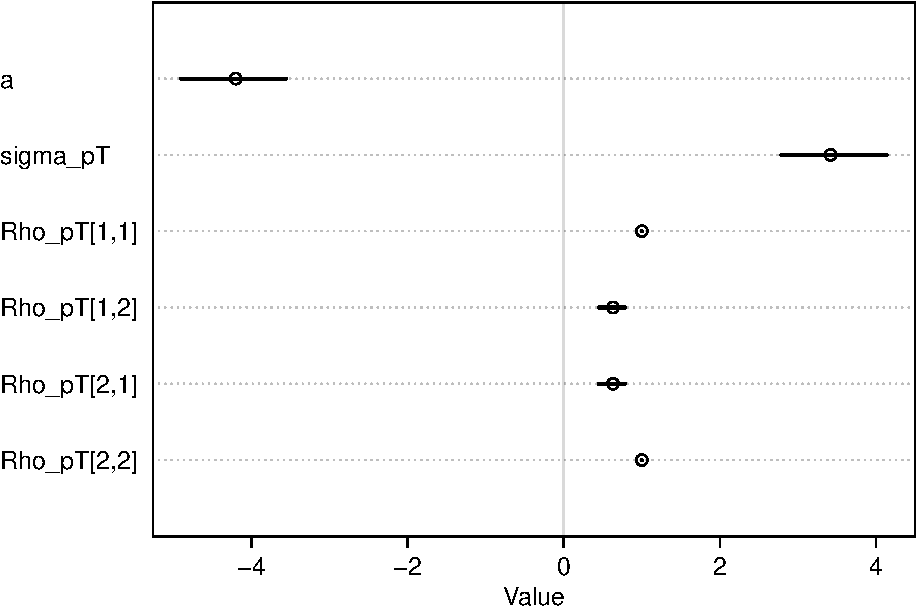
\includegraphics{Geraldes-week08_files/figure-latex/unnamed-chunk-5-1} \end{center}

\begin{Shaded}
\begin{Highlighting}[]
\NormalTok{post.m1 }\OtherTok{\textless{}{-}} \FunctionTok{extract.samples}\NormalTok{(m1)}
\NormalTok{rho\_pt.df }\OtherTok{\textless{}{-}} \FunctionTok{tibble}\NormalTok{(}\AttributeTok{x=}\NormalTok{post.m1}\SpecialCharTok{$}\NormalTok{Rho\_pT[,}\DecValTok{1}\NormalTok{,}\DecValTok{2}\NormalTok{])}
\end{Highlighting}
\end{Shaded}

\begin{center}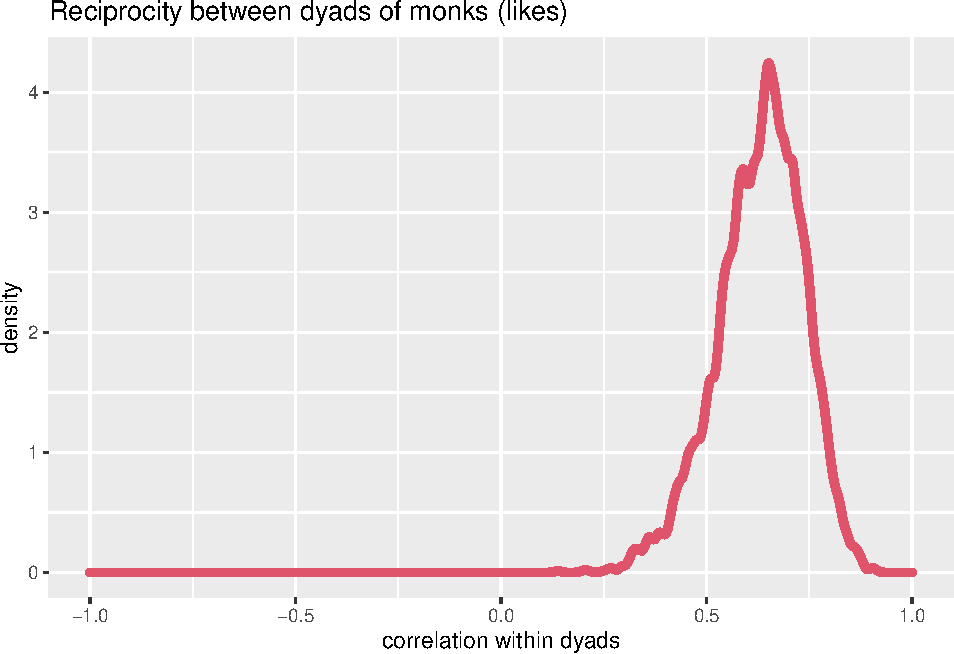
\includegraphics{Geraldes-week08_files/figure-latex/unnamed-chunk-7-1} \end{center}

\hypertarget{question-2}{%
\section{Question 2}\label{question-2}}

Now also analyse the ``dislike'' nominations. Estimate the amount of
reciprocity in the ``dislike'' nominations and compare to the estimate
from the ``like'' nominations. Does ``like'' or ``dislike'' have higher
reciprocity? Be sure to compute the posterior contrast between the two
estimates.

\hypertarget{answer-1}{%
\subsection{Answer}\label{answer-1}}

We define a model where the number of dislike votes from A to B,
\(D_{AB}\) is a binomial distribution of size 3 and probability
\(p_{D_{AB}}\), with symmetric values indexed for the direction
\(B \rightarrow A\). The logit of a \(p_{D_j}\) is the sum of an
intercept \(\alpha\) with an effect of the negative ties \(T^-\) for
\(A \rightarrow B\), correlated to its counterpart for
\(B \rightarrow A\). The priors are fairly flat.

\[
\begin{aligned}
    D_{AB} \sim \text{Binomial}(3, p_{D_{AB}})\\
    D_{BA} \sim \text{Binomial}(3, p_{D_{BA}})\\
    \text{logit}(p_{D_{AB}}) = \alpha + T^-_{AB_i}\\
    \text{logit}(p_{D_{BA}}) = \alpha + T^-_{BA_i}\\
    \alpha \sim \text{Normal}(0,1)\\
    \begin{pmatrix}T^-_{AB}\\T^-_{BA}\end{pmatrix} \sim \text{MVNormal}\begin{pmatrix}\begin{pmatrix}0\\0\end{pmatrix}, \begin{pmatrix}\sigma_{T^-}^2 & \rho_{T^-}\sigma_{T^-}^2\\\rho_{T^-}\sigma_{T^-}^2 &\sigma_{T^-}^2\end{pmatrix}\end{pmatrix}\\
    \sigma_{T^-} \sim \text{Exponential}(1)\\
    \rho_{T^-} \sim \text{LKJCorr}(2)
\end{aligned}
\]

\begin{Shaded}
\begin{Highlighting}[]
\NormalTok{f.m2 }\OtherTok{\textless{}{-}} \FunctionTok{alist}\NormalTok{(}
\NormalTok{    DAB }\SpecialCharTok{\textasciitilde{}} \FunctionTok{binomial}\NormalTok{(}\DecValTok{3}\NormalTok{, pDAB),}
\NormalTok{    DBA }\SpecialCharTok{\textasciitilde{}} \FunctionTok{binomial}\NormalTok{(}\DecValTok{3}\NormalTok{, pDBA),}

    \FunctionTok{logit}\NormalTok{(pDAB) }\OtherTok{\textless{}{-}}\NormalTok{ a }\SpecialCharTok{+}\NormalTok{ nT[D,}\DecValTok{1}\NormalTok{],}
    \FunctionTok{logit}\NormalTok{(pDBA) }\OtherTok{\textless{}{-}}\NormalTok{ a }\SpecialCharTok{+}\NormalTok{ nT[D,}\DecValTok{2}\NormalTok{],}

\NormalTok{    a }\SpecialCharTok{\textasciitilde{}} \FunctionTok{normal}\NormalTok{(}\DecValTok{0}\NormalTok{,}\DecValTok{1}\NormalTok{),}

\NormalTok{    transpars}\SpecialCharTok{\textgreater{}}\NormalTok{ matrix[N,}\DecValTok{2}\NormalTok{]}\SpecialCharTok{:}\NormalTok{nT }\OtherTok{\textless{}{-}} 
        \FunctionTok{compose\_noncentered}\NormalTok{(}\FunctionTok{rep\_vector}\NormalTok{(sigma\_nT, }\DecValTok{2}\NormalTok{), L\_Rho\_nT, z),}
\NormalTok{    matrix[}\DecValTok{2}\NormalTok{,N]}\SpecialCharTok{:}\NormalTok{z }\SpecialCharTok{\textasciitilde{}} \FunctionTok{normal}\NormalTok{(}\DecValTok{0}\NormalTok{,}\DecValTok{1}\NormalTok{),}
\NormalTok{    cholesky\_factor\_corr[}\DecValTok{2}\NormalTok{]}\SpecialCharTok{:}\NormalTok{L\_Rho\_nT }\SpecialCharTok{\textasciitilde{}} \FunctionTok{lkj\_corr\_cholesky}\NormalTok{(}\DecValTok{2}\NormalTok{),}
\NormalTok{    sigma\_nT }\SpecialCharTok{\textasciitilde{}} \FunctionTok{exponential}\NormalTok{(}\DecValTok{1}\NormalTok{),}

\NormalTok{    gq}\SpecialCharTok{\textgreater{}}\NormalTok{ matrix[}\DecValTok{2}\NormalTok{,}\DecValTok{2}\NormalTok{]}\SpecialCharTok{:}\NormalTok{Rho\_nT }\OtherTok{\textless{}\textless{}{-}} \FunctionTok{Chol\_to\_Corr}\NormalTok{(L\_Rho\_nT)}
\NormalTok{)}

\NormalTok{m2 }\OtherTok{\textless{}{-}} \FunctionTok{ulam}\NormalTok{(}
    \AttributeTok{flist =}\NormalTok{ f.m2,}
    \AttributeTok{data =}\NormalTok{ dat,}
    \AttributeTok{chains=}\DecValTok{4}\NormalTok{,}
    \AttributeTok{cores=}\DecValTok{4}\NormalTok{,}
    \AttributeTok{iter=}\DecValTok{2000}\NormalTok{,}
    \AttributeTok{log\_lik=}\ConstantTok{TRUE}\NormalTok{,}
    \AttributeTok{file=}\StringTok{"./models/m2"}\NormalTok{)}
\end{Highlighting}
\end{Shaded}

\begin{Shaded}
\begin{Highlighting}[]
\FunctionTok{precis}\NormalTok{(m2, }\AttributeTok{pars=}\FunctionTok{c}\NormalTok{(}\StringTok{"a"}\NormalTok{, }\StringTok{"sigma\_nT"}\NormalTok{, }\StringTok{"Rho\_nT"}\NormalTok{), }\AttributeTok{depth=}\DecValTok{3}\NormalTok{)}
\end{Highlighting}
\end{Shaded}

\begin{verbatim}
##                   mean        sd       5.5%      94.5%    n_eff     Rhat4
## a           -4.5010766 0.4445605 -5.2409298 -3.8334784 2211.830 0.9997561
## sigma_nT     3.3571202 0.4281518  2.7214834  4.0659510 1526.274 1.0022049
## Rho_nT[1,1]  1.0000000 0.0000000  1.0000000  1.0000000      NaN       NaN
## Rho_nT[1,2]  0.4544655 0.1356955  0.2328227  0.6566736 1072.802 1.0011560
## Rho_nT[2,1]  0.4544655 0.1356955  0.2328227  0.6566736 1072.802 1.0011560
## Rho_nT[2,2]  1.0000000 0.0000000  1.0000000  1.0000000      NaN       NaN
\end{verbatim}

\begin{center}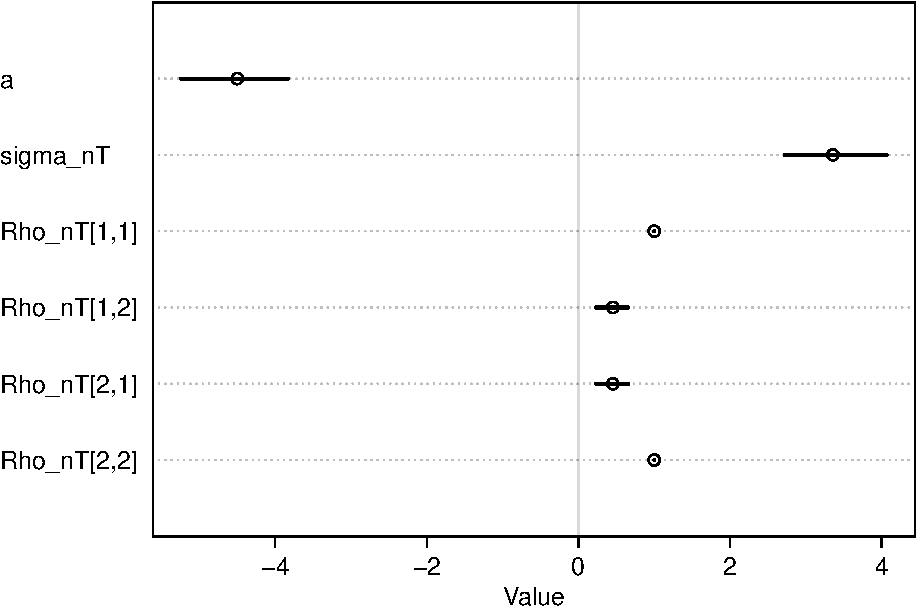
\includegraphics{Geraldes-week08_files/figure-latex/unnamed-chunk-10-1} \end{center}

In this model, the negative ties between any dyad of monks has, on
average, lower reciprocity than the positive ties in the same dyad. But
notice that the overlap is not negligible.

\begin{Shaded}
\begin{Highlighting}[]
\NormalTok{post.m2 }\OtherTok{\textless{}{-}} \FunctionTok{extract.samples}\NormalTok{(m2)}
\NormalTok{rho\_nt.df }\OtherTok{\textless{}{-}} \FunctionTok{tibble}\NormalTok{(}\AttributeTok{x=}\NormalTok{post.m2}\SpecialCharTok{$}\NormalTok{Rho\_nT[,}\DecValTok{1}\NormalTok{,}\DecValTok{2}\NormalTok{])}
\NormalTok{diff.df }\OtherTok{\textless{}{-}} \FunctionTok{tibble}\NormalTok{(}\AttributeTok{x=}\NormalTok{rho\_pt.df}\SpecialCharTok{$}\NormalTok{x }\SpecialCharTok{{-}}\NormalTok{ rho\_nt.df}\SpecialCharTok{$}\NormalTok{x)}
\end{Highlighting}
\end{Shaded}

\begin{center}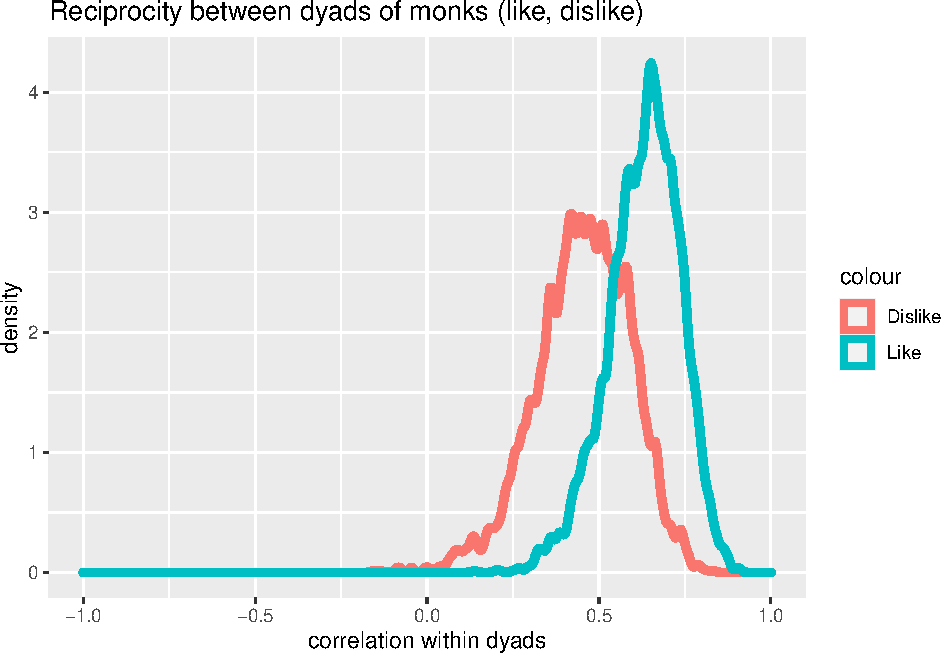
\includegraphics{Geraldes-week08_files/figure-latex/unnamed-chunk-12-1} \end{center}

\begin{center}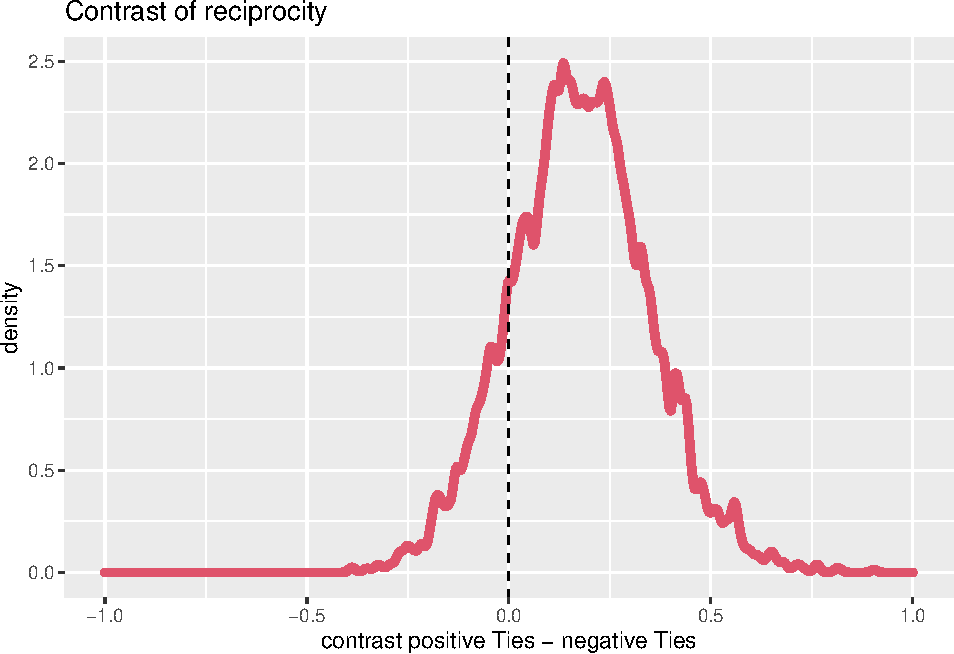
\includegraphics{Geraldes-week08_files/figure-latex/unnamed-chunk-12-2} \end{center}

\hypertarget{question-3}{%
\section{Question 3}\label{question-3}}

Now consider generalized liking and disliking. Add generalized
``receiving'' parameters to the model, analogous to receiving varying
effects from the sharing example in the book/lecture. (Each monk only
named 3 likes and 3 dislikes each time, so the amount of ``giving'' is
fixed by design in these data.) Can you identify any individuals who are
particularly liked/disliked, independent of the dyadic relations?

\hypertarget{answer-2}{%
\subsection{Answer}\label{answer-2}}

\[
\begin{aligned}
    L_{AB} \sim \text{Binomial}(3, p_{L_{AB}})\\
    L_{BA} \sim \text{Binomial}(3, p_{L_{BA}})\\
    D_{AB} \sim \text{Binomial}(3, p_{D_{AB}})\\
    D_{BA} \sim \text{Binomial}(3, p_{D_{BA}})\\
    \text{logit}(p_{L_{AB}}) = \alpha_L + T^+_{AB_i} + R_{LB_i}\\
    \text{logit}(p_{L_{BA}}) = \alpha_L + T^+_{BA_i} + R_{LA_i}\\
    \text{logit}(p_{D_{AB}}) = \alpha + T^-_{AB_i} + R_{DB_i}\\
    \text{logit}(p_{D_{BA}}) = \alpha + T^-_{BA_i} + R_{DA_i}\\
    \alpha_j \sim \text{Normal}(0,1)\\
    \begin{pmatrix}T^+_{AB}\\T^+_{BA}\end{pmatrix} \sim \text{MVNormal}\begin{pmatrix}\begin{pmatrix}0\\0\end{pmatrix}, \textbf{S}_{T^+}, \textbf{R}_{T^+}\end{pmatrix}\\
    \begin{pmatrix}T^-_{AB}\\T^-_{BA}\end{pmatrix} \sim \text{MVNormal}\begin{pmatrix}\begin{pmatrix}0\\0\end{pmatrix}, \textbf{S}_{T^-}, \textbf{R}_{T^-}\end{pmatrix}\\
    \begin{pmatrix}R_{Lj}\\R_{Dj}\end{pmatrix} \sim \text{MVNormal}\begin{pmatrix}\begin{pmatrix}0\\0\end{pmatrix}, \textbf{S}_{LD}, \textbf{R}_{LD}\end{pmatrix}\\
    \textbf{S}_{T^+}, \textbf{S}_{T^-}, \textbf{S}_{LD} \sim \text{Exponential}(1)\\
    \textbf{R}_{T^+}, \textbf{R}_{T^-}, \textbf{R}_{LD} \sim \text{LKJCorr}(2)
\end{aligned}
\]

\begin{Shaded}
\begin{Highlighting}[]
\NormalTok{f.m6 }\OtherTok{\textless{}{-}} \FunctionTok{alist}\NormalTok{(}
\NormalTok{    LAB }\SpecialCharTok{\textasciitilde{}} \FunctionTok{binomial}\NormalTok{(}\DecValTok{3}\NormalTok{, pLAB),}
\NormalTok{    LBA }\SpecialCharTok{\textasciitilde{}} \FunctionTok{binomial}\NormalTok{(}\DecValTok{3}\NormalTok{, pLBA),}
\NormalTok{    DAB }\SpecialCharTok{\textasciitilde{}} \FunctionTok{binomial}\NormalTok{(}\DecValTok{3}\NormalTok{, pDAB),}
\NormalTok{    DBA }\SpecialCharTok{\textasciitilde{}} \FunctionTok{binomial}\NormalTok{(}\DecValTok{3}\NormalTok{, pDBA),}

    \FunctionTok{logit}\NormalTok{(pLAB) }\OtherTok{\textless{}{-}}\NormalTok{ a[}\DecValTok{1}\NormalTok{] }\SpecialCharTok{+}\NormalTok{ pT[D,}\DecValTok{1}\NormalTok{] }\SpecialCharTok{+}\NormalTok{ rlrd[mB,}\DecValTok{1}\NormalTok{],}
    \FunctionTok{logit}\NormalTok{(pLBA) }\OtherTok{\textless{}{-}}\NormalTok{ a[}\DecValTok{1}\NormalTok{] }\SpecialCharTok{+}\NormalTok{ pT[D,}\DecValTok{2}\NormalTok{] }\SpecialCharTok{+}\NormalTok{ rlrd[mA,}\DecValTok{1}\NormalTok{],}
    \FunctionTok{logit}\NormalTok{(pDAB) }\OtherTok{\textless{}{-}}\NormalTok{ a[}\DecValTok{2}\NormalTok{] }\SpecialCharTok{+}\NormalTok{ nT[D,}\DecValTok{1}\NormalTok{] }\SpecialCharTok{+}\NormalTok{ rlrd[mB,}\DecValTok{2}\NormalTok{],}
    \FunctionTok{logit}\NormalTok{(pDBA) }\OtherTok{\textless{}{-}}\NormalTok{ a[}\DecValTok{2}\NormalTok{] }\SpecialCharTok{+}\NormalTok{ nT[D,}\DecValTok{2}\NormalTok{] }\SpecialCharTok{+}\NormalTok{ rlrd[mA,}\DecValTok{2}\NormalTok{],}

\NormalTok{    vector[}\DecValTok{2}\NormalTok{]}\SpecialCharTok{:}\NormalTok{a }\SpecialCharTok{\textasciitilde{}} \FunctionTok{normal}\NormalTok{(}\DecValTok{0}\NormalTok{, }\DecValTok{1}\NormalTok{),}

\NormalTok{    transpars}\SpecialCharTok{\textgreater{}}\NormalTok{matrix[}\DecValTok{18}\NormalTok{,}\DecValTok{2}\NormalTok{]}\SpecialCharTok{:}\NormalTok{rlrd }\OtherTok{\textless{}{-}} 
        \FunctionTok{compose\_noncentered}\NormalTok{(}\FunctionTok{rep\_vector}\NormalTok{(sigma\_rlrd, }\DecValTok{2}\NormalTok{), L\_Rho\_rlrd, zR),}
\NormalTok{    matrix[}\DecValTok{2}\NormalTok{,}\DecValTok{18}\NormalTok{]}\SpecialCharTok{:}\NormalTok{zR }\SpecialCharTok{\textasciitilde{}} \FunctionTok{normal}\NormalTok{(}\DecValTok{0}\NormalTok{,}\DecValTok{1}\NormalTok{),}
\NormalTok{    cholesky\_factor\_corr[}\DecValTok{2}\NormalTok{]}\SpecialCharTok{:}\NormalTok{L\_Rho\_rlrd }\SpecialCharTok{\textasciitilde{}} \FunctionTok{lkj\_corr\_cholesky}\NormalTok{(}\DecValTok{2}\NormalTok{),}
\NormalTok{    sigma\_rlrd }\SpecialCharTok{\textasciitilde{}} \FunctionTok{exponential}\NormalTok{(}\DecValTok{1}\NormalTok{),}

\NormalTok{    transpars}\SpecialCharTok{\textgreater{}}\NormalTok{ matrix[N,}\DecValTok{2}\NormalTok{]}\SpecialCharTok{:}\NormalTok{pT }\OtherTok{\textless{}{-}} 
        \FunctionTok{compose\_noncentered}\NormalTok{(}\FunctionTok{rep\_vector}\NormalTok{(sigma\_pT, }\DecValTok{2}\NormalTok{), L\_Rho\_pT, zP),}
\NormalTok{    matrix[}\DecValTok{2}\NormalTok{,N]}\SpecialCharTok{:}\NormalTok{zP }\SpecialCharTok{\textasciitilde{}} \FunctionTok{normal}\NormalTok{(}\DecValTok{0}\NormalTok{,}\DecValTok{1}\NormalTok{),}
\NormalTok{    cholesky\_factor\_corr[}\DecValTok{2}\NormalTok{]}\SpecialCharTok{:}\NormalTok{L\_Rho\_pT }\SpecialCharTok{\textasciitilde{}} \FunctionTok{lkj\_corr\_cholesky}\NormalTok{(}\DecValTok{2}\NormalTok{),}
\NormalTok{    sigma\_pT }\SpecialCharTok{\textasciitilde{}} \FunctionTok{exponential}\NormalTok{(}\DecValTok{1}\NormalTok{),}

\NormalTok{    transpars}\SpecialCharTok{\textgreater{}}\NormalTok{ matrix[N,}\DecValTok{2}\NormalTok{]}\SpecialCharTok{:}\NormalTok{nT }\OtherTok{\textless{}{-}} 
        \FunctionTok{compose\_noncentered}\NormalTok{(}\FunctionTok{rep\_vector}\NormalTok{(sigma\_nT, }\DecValTok{2}\NormalTok{), L\_Rho\_nT, zN),}
\NormalTok{    matrix[}\DecValTok{2}\NormalTok{,N]}\SpecialCharTok{:}\NormalTok{zN }\SpecialCharTok{\textasciitilde{}} \FunctionTok{normal}\NormalTok{(}\DecValTok{0}\NormalTok{,}\DecValTok{1}\NormalTok{),}
\NormalTok{    cholesky\_factor\_corr[}\DecValTok{2}\NormalTok{]}\SpecialCharTok{:}\NormalTok{L\_Rho\_nT }\SpecialCharTok{\textasciitilde{}} \FunctionTok{lkj\_corr\_cholesky}\NormalTok{(}\DecValTok{2}\NormalTok{),}
\NormalTok{    sigma\_nT }\SpecialCharTok{\textasciitilde{}} \FunctionTok{exponential}\NormalTok{(}\DecValTok{1}\NormalTok{),}

\NormalTok{    gq}\SpecialCharTok{\textgreater{}}\NormalTok{ matrix[}\DecValTok{2}\NormalTok{,}\DecValTok{2}\NormalTok{]}\SpecialCharTok{:}\NormalTok{Rho\_pT }\OtherTok{\textless{}\textless{}{-}} \FunctionTok{Chol\_to\_Corr}\NormalTok{(L\_Rho\_pT),}
\NormalTok{    gq}\SpecialCharTok{\textgreater{}}\NormalTok{ matrix[}\DecValTok{2}\NormalTok{,}\DecValTok{2}\NormalTok{]}\SpecialCharTok{:}\NormalTok{Rho\_nT }\OtherTok{\textless{}\textless{}{-}} \FunctionTok{Chol\_to\_Corr}\NormalTok{(L\_Rho\_nT),}
\NormalTok{    gq}\SpecialCharTok{\textgreater{}}\NormalTok{ matrix[}\DecValTok{2}\NormalTok{,}\DecValTok{2}\NormalTok{]}\SpecialCharTok{:}\NormalTok{Rho\_rlrd }\OtherTok{\textless{}\textless{}{-}} \FunctionTok{Chol\_to\_Corr}\NormalTok{(L\_Rho\_rlrd)}
\NormalTok{)}

\NormalTok{m6 }\OtherTok{\textless{}{-}} \FunctionTok{ulam}\NormalTok{(}\AttributeTok{flist =}\NormalTok{ f.m6, }
           \AttributeTok{data=}\NormalTok{dat, }
           \AttributeTok{cores=}\DecValTok{4}\NormalTok{,}
           \AttributeTok{chains=}\DecValTok{4}\NormalTok{,}
           \AttributeTok{iter=}\DecValTok{2000}\NormalTok{,}
           \AttributeTok{log\_lik=}\ConstantTok{TRUE}\NormalTok{,}
           \AttributeTok{file=}\StringTok{"./models/m6"}\NormalTok{)}
\end{Highlighting}
\end{Shaded}

\begin{Shaded}
\begin{Highlighting}[]
\FunctionTok{precis}\NormalTok{(m6, }\AttributeTok{pars=}\FunctionTok{c}\NormalTok{(}\StringTok{"a"}\NormalTok{, }\StringTok{"sigma\_pT"}\NormalTok{, }\StringTok{"sigma\_nT"}\NormalTok{, }\StringTok{"sigma\_rlrd"}\NormalTok{,}
                  \StringTok{"Rho\_pT"}\NormalTok{, }\StringTok{"Rho\_nT"}\NormalTok{, }\StringTok{"Rho\_rlrd"}\NormalTok{), }\AttributeTok{depth=}\DecValTok{3}\NormalTok{)}
\end{Highlighting}
\end{Shaded}

\begin{verbatim}
##                     mean        sd       5.5%      94.5%     n_eff     Rhat4
## a[1]          -3.6831612 0.7319731 -4.7309827 -2.3836368 1043.3204 0.9996800
## a[2]          -3.7481130 0.7097196 -4.7458697 -2.5128470 1333.0989 0.9997903
## sigma_pT       3.6314505 0.5081121  2.8849677  4.4842843 1623.1561 1.0013524
## sigma_nT       2.9196465 0.4117690  2.3236229  3.5991569 1485.5946 1.0016727
## sigma_rlrd     1.9339893 0.7000080  1.1007613  3.2416830  689.8158 1.0011356
## Rho_pT[1,1]    1.0000000 0.0000000  1.0000000  1.0000000       NaN       NaN
## Rho_pT[1,2]    0.6650927 0.1083009  0.4788825  0.8223094 1613.8831 0.9994749
## Rho_pT[2,1]    0.6650927 0.1083009  0.4788825  0.8223094 1613.8831 0.9994749
## Rho_pT[2,2]    1.0000000 0.0000000  1.0000000  1.0000000       NaN       NaN
## Rho_nT[1,1]    1.0000000 0.0000000  1.0000000  1.0000000       NaN       NaN
## Rho_nT[1,2]    0.5350608 0.1542301  0.2710096  0.7665078 1342.0602 1.0010733
## Rho_nT[2,1]    0.5350608 0.1542301  0.2710096  0.7665078 1342.0602 1.0010733
## Rho_nT[2,2]    1.0000000 0.0000000  1.0000000  1.0000000       NaN       NaN
## Rho_rlrd[1,1]  1.0000000 0.0000000  1.0000000  1.0000000       NaN       NaN
## Rho_rlrd[1,2]  0.1153858 0.3440382 -0.4406062  0.6601409  791.3867 1.0005227
## Rho_rlrd[2,1]  0.1153858 0.3440382 -0.4406062  0.6601409  791.3867 1.0005227
## Rho_rlrd[2,2]  1.0000000 0.0000000  1.0000000  1.0000000       NaN       NaN
\end{verbatim}

\begin{center}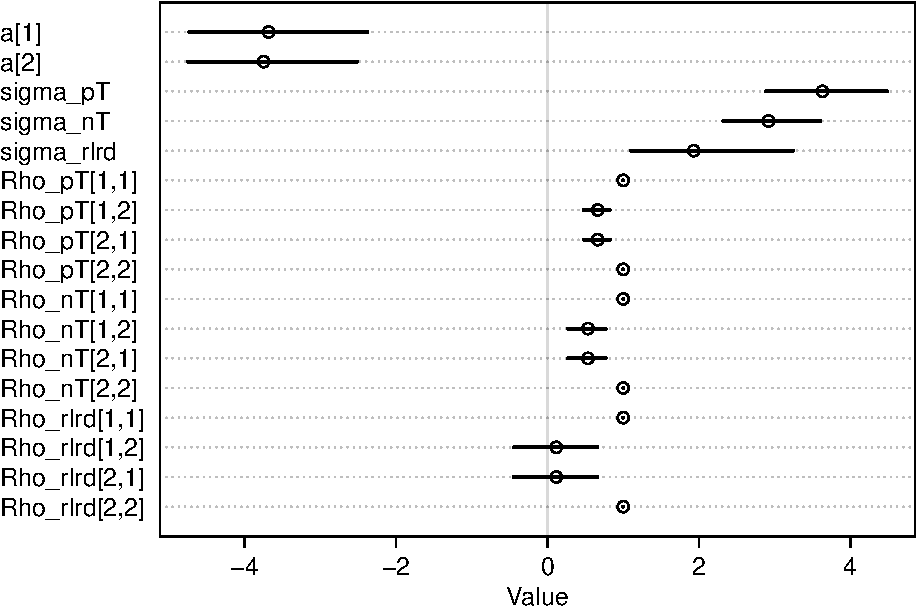
\includegraphics{Geraldes-week08_files/figure-latex/unnamed-chunk-15-1} \end{center}

The average reciprocity of negative and positive ties has remained
fairly similar to the previous model.

\begin{Shaded}
\begin{Highlighting}[]
\NormalTok{post.m6 }\OtherTok{\textless{}{-}} \FunctionTok{extract.samples}\NormalTok{(m6)}
\NormalTok{m6.df }\OtherTok{\textless{}{-}} \FunctionTok{tibble}\NormalTok{(}\AttributeTok{pt=}\NormalTok{post.m6}\SpecialCharTok{$}\NormalTok{Rho\_pT[,}\DecValTok{1}\NormalTok{,}\DecValTok{2}\NormalTok{],}
                \AttributeTok{nt=}\NormalTok{post.m6}\SpecialCharTok{$}\NormalTok{Rho\_nT[,}\DecValTok{1}\NormalTok{,}\DecValTok{2}\NormalTok{],}
                \AttributeTok{rlrd=}\NormalTok{post.m6}\SpecialCharTok{$}\NormalTok{Rho\_rlrd[,}\DecValTok{1}\NormalTok{,}\DecValTok{2}\NormalTok{]) }\SpecialCharTok{\%\textgreater{}\%}
  \FunctionTok{mutate}\NormalTok{(}\AttributeTok{difft =}\NormalTok{ pt}\SpecialCharTok{{-}}\NormalTok{nt)}
\end{Highlighting}
\end{Shaded}

\begin{center}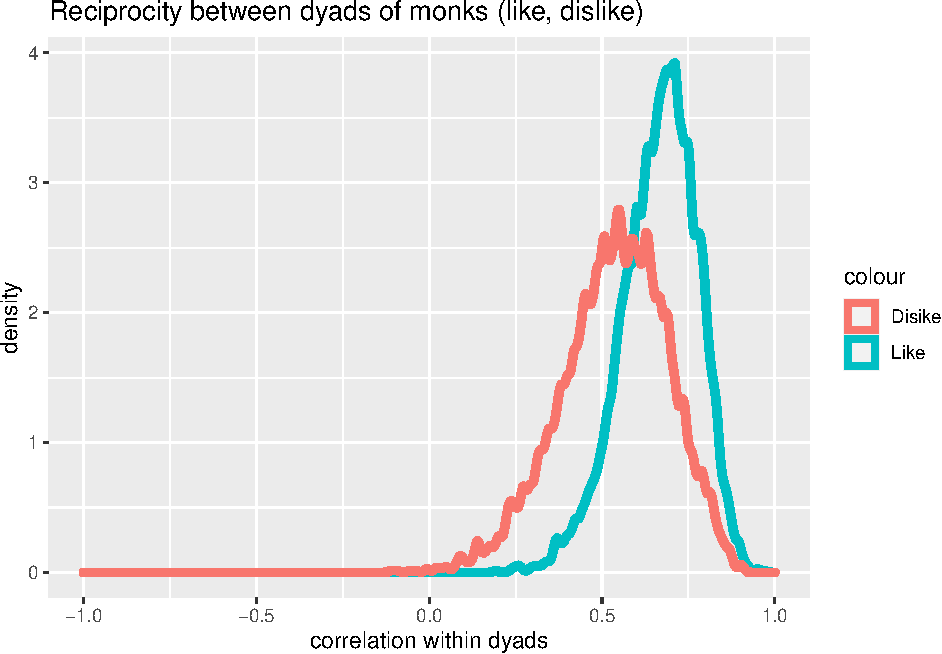
\includegraphics{Geraldes-week08_files/figure-latex/unnamed-chunk-17-1} \end{center}

\begin{center}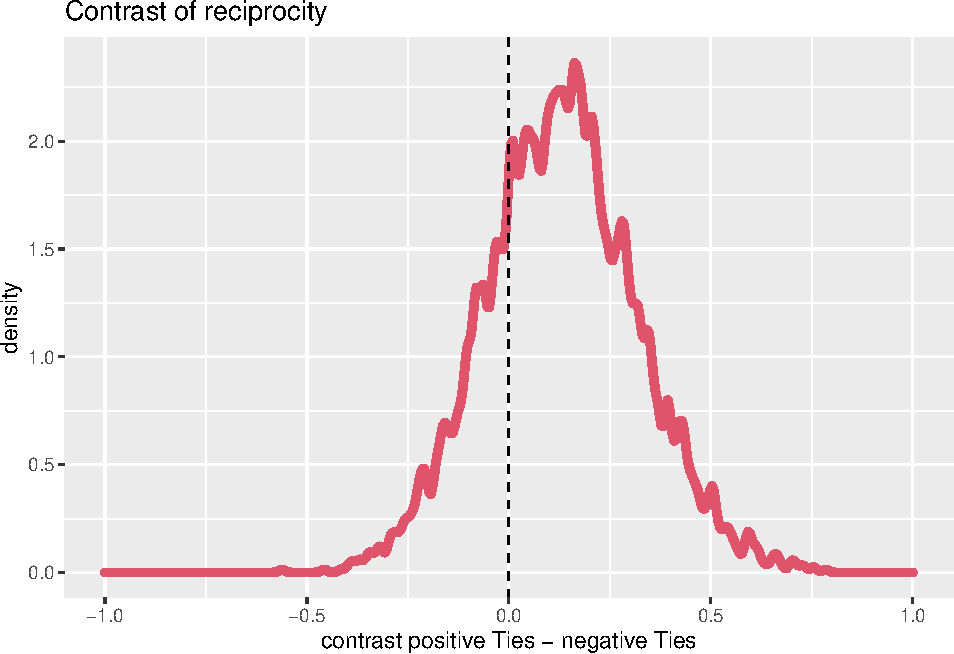
\includegraphics{Geraldes-week08_files/figure-latex/unnamed-chunk-17-2} \end{center}

\begin{center}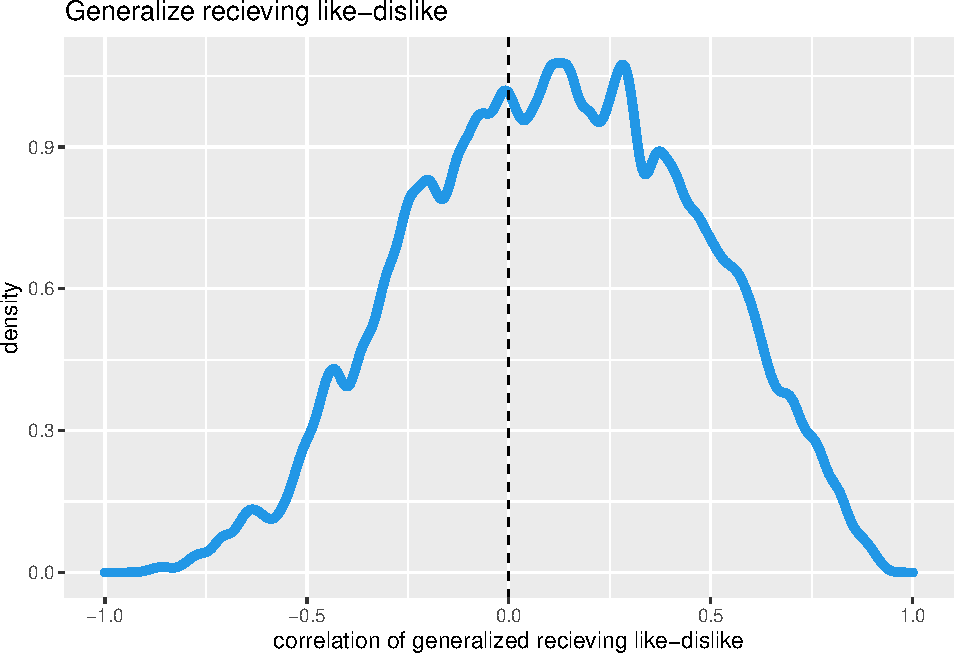
\includegraphics{Geraldes-week08_files/figure-latex/unnamed-chunk-17-3} \end{center}

There are some monks whose dislike-like ratio seems to be very far from
average, and the model is very uncertain about how far they actually
are. Peter, Greg, Victor and Basil have highly above average dislike
odds, and although the model is uncertain of how much disliked they
actually are, they certainly fall above the like=dislike line. Boni and
Bonaven are quite liked according to the model, but the model is much
less certain if they are actually unevenly liked or disliked: the model
is confident that they are not hated at all costs, but is not so sure
about their charisma.

\begin{Shaded}
\begin{Highlighting}[]
\NormalTok{monknames }\OtherTok{\textless{}{-}}\NormalTok{ (monks }\SpecialCharTok{\%\textgreater{}\%}
                  \FunctionTok{select}\NormalTok{(B, B\_name) }\SpecialCharTok{\%\textgreater{}\%} 
                  \FunctionTok{distinct}\NormalTok{() }\SpecialCharTok{\%\textgreater{}\%}
                  \FunctionTok{add\_row}\NormalTok{(}\AttributeTok{B=}\DecValTok{1}\NormalTok{, }\AttributeTok{B\_name=}\StringTok{"ROMUL"}\NormalTok{) }\SpecialCharTok{\%\textgreater{}\%}
                  \FunctionTok{arrange}\NormalTok{(B))}\SpecialCharTok{$}\NormalTok{B\_name}

\NormalTok{l }\OtherTok{\textless{}{-}} \FunctionTok{sapply}\NormalTok{(}\DecValTok{1}\SpecialCharTok{:}\DecValTok{18}\NormalTok{, }\ControlFlowTok{function}\NormalTok{(i) post.m6}\SpecialCharTok{$}\NormalTok{a[,}\DecValTok{1}\NormalTok{] }\SpecialCharTok{+}\NormalTok{ post.m6}\SpecialCharTok{$}\NormalTok{rlrd[,i,}\DecValTok{1}\NormalTok{])}
\NormalTok{d }\OtherTok{\textless{}{-}} \FunctionTok{sapply}\NormalTok{(}\DecValTok{1}\SpecialCharTok{:}\DecValTok{18}\NormalTok{, }\ControlFlowTok{function}\NormalTok{(i) post.m6}\SpecialCharTok{$}\NormalTok{a[,}\DecValTok{2}\NormalTok{] }\SpecialCharTok{+}\NormalTok{ post.m6}\SpecialCharTok{$}\NormalTok{rlrd[,i,}\DecValTok{2}\NormalTok{])}
\NormalTok{l\_mu }\OtherTok{\textless{}{-}} \FunctionTok{apply}\NormalTok{(}\FunctionTok{inv\_logit}\NormalTok{(l), }\DecValTok{2}\NormalTok{, mean)}
\NormalTok{d\_mu }\OtherTok{\textless{}{-}} \FunctionTok{apply}\NormalTok{(}\FunctionTok{inv\_logit}\NormalTok{(d), }\DecValTok{2}\NormalTok{, mean)}

\NormalTok{ld.df }\OtherTok{\textless{}{-}} \FunctionTok{tibble}\NormalTok{(}\AttributeTok{monk=}\NormalTok{monknames, }\AttributeTok{like=}\NormalTok{l\_mu, }\AttributeTok{dislike=}\NormalTok{d\_mu)}
\end{Highlighting}
\end{Shaded}

\begin{center}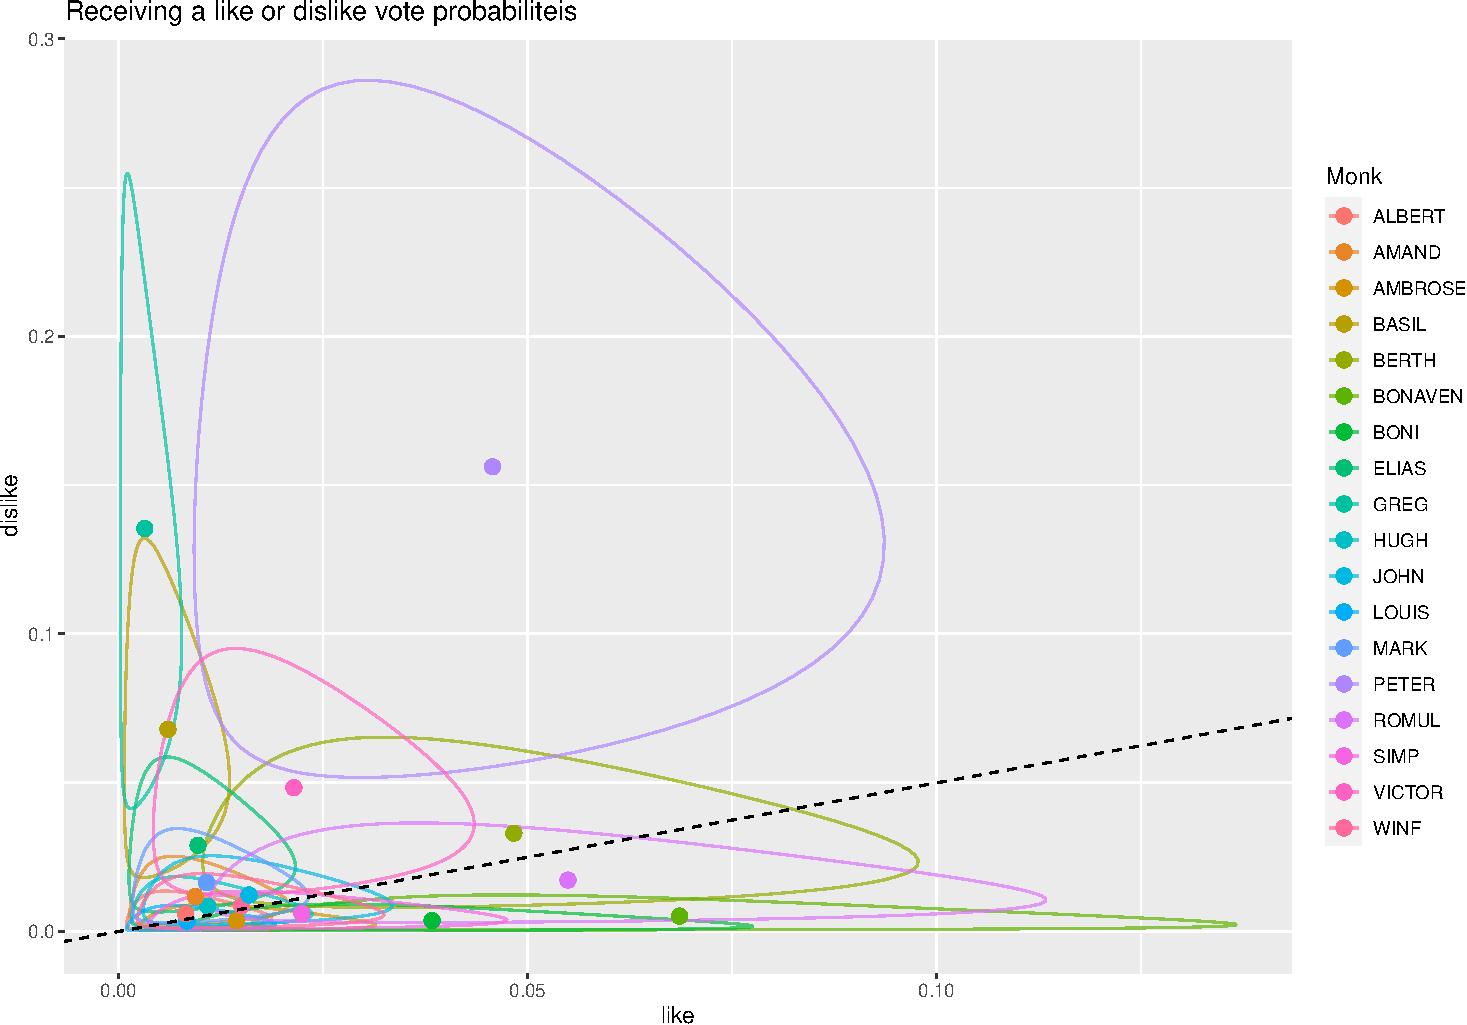
\includegraphics{Geraldes-week08_files/figure-latex/unnamed-chunk-19-1} \end{center}

\end{document}
